\subsection{GR4J (model ID: 07)}
The GR4J model (fig.~\ref{fig:07_schematic}) is originally developed with an explicit (operator-splitting) time-stepping scheme \citep{Perrin2003}. Recently a new version has been released that works with an implicit time-stepping scheme \citep{Santos2017}. The implementation given here follows most of the equations from \citet{Santos2017}, but uses the original Unit Hydrographs for flood routing given by \citet{Perrin2003}. It has 2 stores and 4 parameters ($x_1$, $x_2$, $x_3$, $x_4$). The model aims to represent:

\begin{itemizecompact}
\item Implicit interception by vegetation, expressed as net precipitation or evaporation;
\item Different time delays within the catchment expressed by two hydrographs;
\item Water exchange with neighbouring catchments.
\end{itemizecompact}

\subsubsection{File names}
\begin{tabular}{@{}ll}
Model: &m\_07\_gr4j\_4p\_2s \\
Parameter ranges: &m\_07\_gr4j\_4p\_2s\_parameter\_ ranges \\
\end{tabular}

% Equations
\subsubsection{Model equations}

% Model layout figure
{ 																	% This ensures it doesn't warp text further down
\begin{wrapfigure}{l}{5cm}
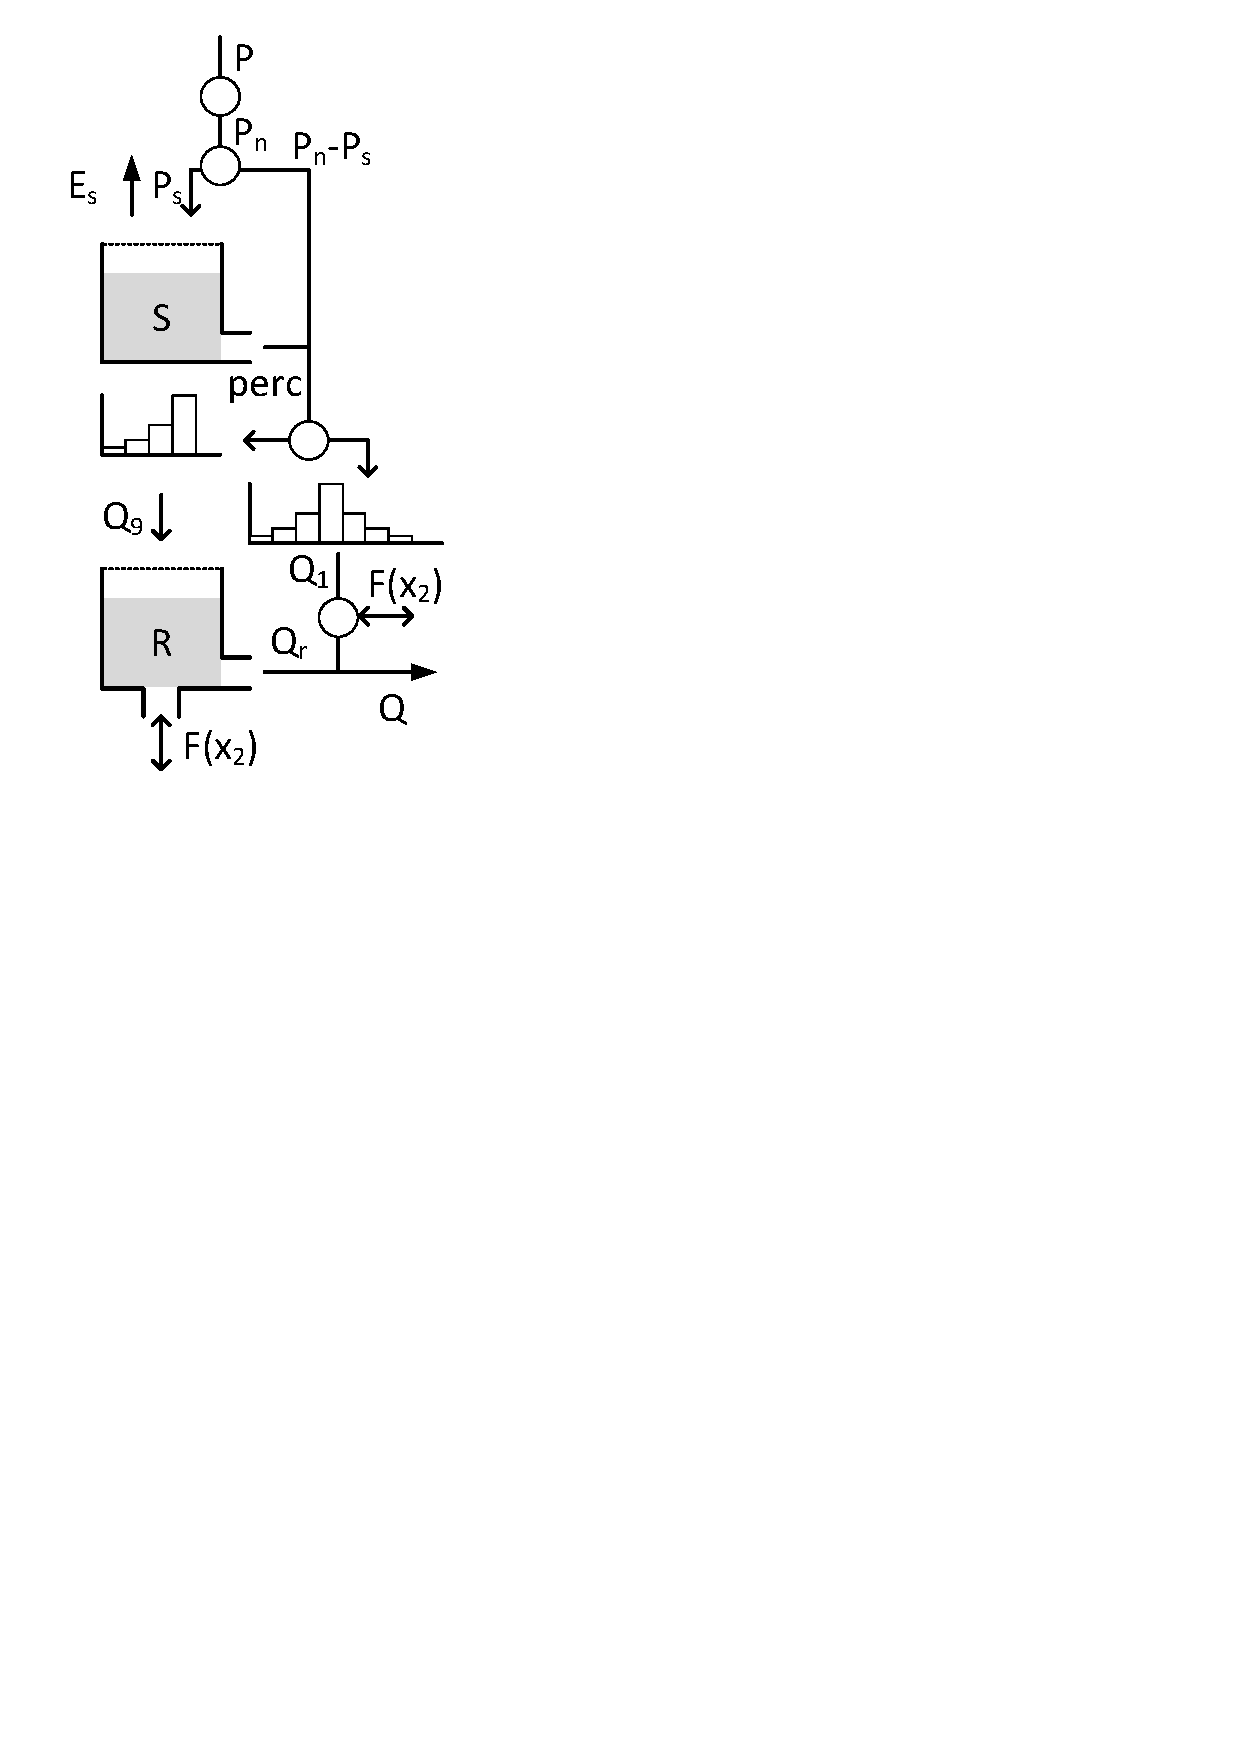
\includegraphics[trim=1cm 17cm 7cm 1cm,width=8cm,keepaspectratio]{./files/07_schematic.pdf}
\caption{Structure of the GR4J model} \label{fig:07_schematic}
\end{wrapfigure}

\begin{align}
	\frac{dS}{dt} &= P_s-E_s-Perc \\
	P_s &= P_n* \left(1-\left(\frac{S}{x1}\right)^2\right)\\
	P_n &= 
	\begin{cases}
		P-Ep, & \text{if } P \geq Ep \\
		0, & \text{otherwise}
	\end{cases} \\
	E_s &= E_n*\left(2\frac{S}{x1}-\left(\frac{S}{x1}\right)^2\right)\\
	E_n &= 
	\begin{cases}
		Ep-P, & \text{if } Ep > P \\
		0, & \text{otherwise}
	\end{cases} \\
	Perc &= \frac{x_1^{-4}}{4}*\left(\frac{4}{9}\right)^{-4}S^5
\end{align}

Where S is the current soil moisture storage [mm], $P_s$ $[mm/d]$ is the fraction of net precipitation $P_n$ $[mm/d]$ redirected to soil moisture, $E_s$ $[mm/d]$ is the fraction of net evaporation $E_n$ $[mm/d]$ subtracted from soil moisture, and $perc$ $[mm/d]$ is percolation to deeper soil layers. Parameter $x_1$ [mm] is the maximum soil moisture storage.

} % end of wrapfigure fix

Percolation $perc$ and excess precipitation $P_n - P_s$ are divided into 90\% groundwater flow, routed through a triangular routing scheme with time base $x_4$ [d], and 10\% direct runoff, routed through a triangular routing scheme with time base $2x_4$ [d].

\begin{align}
	\frac{dR}{dt} &= Q_{9} + F(x_2) -Q_r\\
	F(x_2) &= x_2*\left(\frac{R}{x_3}\right)^{3.5} \\	
	Q_r &= \frac{x_3^{-4}}{4}R^5
\end{align}

Where $R$ [mm] is the current storage in the routing store, $F(x_2)$ $[mm/d]$ the catchment groundwater exchange, depending on exchange coefficient $x_2$ $[mm/d]$ and the maximum routing capacity $x_3$ [mm], and $Q_r$ $[mm/d]$ routed flow. Total runoff $Q_t$ $[mm/d]$: 

\begin{equation}
	Q_t = Q_r + max(Q_1+F(x_2),0)
\end{equation} 

\subsubsection{Parameter overview}
% Table generated by Excel2LaTeX from sheet 'Sheet1'
\begin{table}[htbp]
  \centering
    \begin{tabular}{lll}
    \toprule
    Parameter & Unit  & Description \\
    \midrule
    $x_1$ & $mm$  & Maximum soil moisture storage \\
    $x_2$ & $mm~d^{-1}$ & Subsurface water exchange \\
    $x_3$ & $mm$  & Routing store depth \\
    $x_4$ & $d$   & Unit Hydrograph time base \\
    \bottomrule
    \end{tabular}%
  \label{tab:addlabel}%
\end{table}%

